% Chapter 3

\chapter{Concept} % Write in your own chapter title
\label{Chapter3}
\lhead{Chapter 3. \emph{Concept}} % Write in your own chapter title to set the page header

From a high point of view SPolly is divided into a speculative loop parallelizer 
and a non speculative extension to Polly. Even if the objectives for both parts 
are the same, namely to improve the performance of loops, the approaches to accomplish 
them are different. While the former one will introduce speculative parallelism
for promising loops at runtime, the later one tries to weaken the harsh 
requirements on SCoPs in order to make Pollys loop optimizations applicable on
a wider range of loop nests. In the presented setting both approaches may benefit
from the polyhedral optimizations and also from parallel execution, so it is 
hardly surprising that the polyhedral analyses play a decisive role. 
On the one hand they reveal loop nests which may be optimized by Polly, with or
without the extensions of SPolly, on the other hand they are used to detect 
promising loops to speculate on.
Apart from the implementation work, which will be described in the 
next chapter, this thesis presents the concepts and key ideas behind.
We believe that these ideas and the gained knowledge is very 
valuable not only for future work on SPolly or one of its bases but also for
other approaches facing similar situations.

%On the way to a working version 
%many pitfalls have been encountered that should be avoided in the future, 
%perhaps with similar approaches we worked out. 


\section{Speculative Parallel Execution}
\label{SpeculativeParallelExecution}
Speculatively executing loops in parallel is one of the two major purposes of 
SPolly. The challenge was to exploit as much parallelism as possible 
without restricting the applicability to much. 

\subsection{Semantic Preservation}
Dven if the execution is secured by a (not extended) STM it may not 
be sound to execute a loop nest in parallel. 
If there is a conflict between two iterations and the
later one (in terms of the original ordering) commits its result before the 
former one could, the STM will force the former one to recompute, 
but now based on corrupted data already committed and therefore permanently written.
From this fact the need of an commit order arose, as it would in any case preserve
the initial ordering when applying permanent changes.

As one great feature of Polly and the underlying polyhedral model
is to detect and model loop carried data dependencies, it sounds plausible to
use this for speculative execution purposes as well. Unfortunately speculative 
extensions will compromise this ability because they will speculatively assume less
dependencies in order to weaken the requirements. 
To handle such situations SPolly tries to unify both of its parts. 
At first, non computable memory accesses, as they arise from 
aliases we cannot check in beforehand or from function calls within a SCoP, are
overestimated. The resulting polyhedral model is complete with regards to possible
data dependencies, but could anyway reveal transformations for a 
better data-locality or possible vectorization. 
Afterwards speculation is applied, thus the optimized loop nest is
speculatively  parallelized. Note here, that only Polly could change the iteration 
order but because this would be based on a complete and overestimated polyhedral model, 
it would still yield a sound ordering. 

In the worst case there are dependencies between all parallel executed iterations
and each thread has to recompute its part once another one committed its results.
As countermeasure to such time consuming misspeculations SPolly monitors 
the runtime of all speculatively parallelized SCoPs and reverts the speculation 
for poorly performing ones.

In contrast to the speculation free optimization approach, this one is also
capable of parallelizing sSCoPs with almost arbitrary function calls. To do so the
STM has to provide the  wait construct as described earlier. 
Even if this is not yet the case, SPolly could introducing such wait with no further effort. 
This will certainly cause additional overhead during the parallel execution, 
but it does not preclude a performance gain per se.

In the special case of sSCoPs, we know certain things about the 
control flow and the memory accesses within a parallelized region. 
With the assumptions we may derive from the requirements on sSCoPs it is possible
to secure the speculative parallel execution by introducing wait constructs 
right before each possibly violating function call. Executing those function calls
in the correct ordering will enforce all their possible effects to be applied 
in the correct order too. 
If arbitrary control flow and conditionals are allowed, this conclusion does not
hold anymore. In fact every memory access could change the taken execution path of 
another thread, thus every branch would need annotation. 



\section{Speculation Free Optimizations}
\label{SpeculationFreesSCoPs}
As second objective SPolly may enable sound polyhedral optimizations, even
parallelization, on sSCoPs with no need for speculation at all. This is the case
when the tests we introduce in the following can rule out all violations of a
sSCoP. 





\section{SPolly In A Nutshell}
%SPolly, as presented here, is composed of a compile time and a runtime part. 
%Their respective tasks are related but not the same. During both steps the, so
%called, region speculation is used to interact with Polly. 
%It is also the 
%part of SPolly which is not integrated  into the Sambamba framework. As some
%of the functionalities do not rely on speculation, it is possible to integrate
%them into the main application of Polly anytime soon. 

%\paragraph{Compile Time }~\\
\begin{wrapfigure}[]{r}{0.4\textwidth}
  \centering
  \vspace*{-2mm}
  \includegraphics[width=0.4\textwidth]{Figures/draftPaperCT.eps}
  \caption{Draft paper: \\SPolly at compile time}
  \vspace*{-5mm}
  \label{fig:draftPaperCT}  
\end{wrapfigure}
During \textbf{compile time} the main goal of SPolly is to simplify the runtime part,
thus to reduce runtime overhead through preprocessing and even static method versioning.
First the SCoP detection tries to find valid regions within the given LLVM-IR, 
but instead of rejecting a region once a restriction is violated, 
the region speculation is asked how to proceed. Restrictions we want to speculate
on are gathered by the region speculation, but ignored by the SCoP detection.
This proceeding allows to find all violations with a region and to treat valid and
speculatively valid ones nearly the same. After all  
speculative valid SCoPs (or short sSCoPs) are encountered the Sambamba compile 
time part takes action. It separates the sSCoPs as some of them do not need
speculation at all. Those sSCoPs are optimized and exchanged, 
while the others are currently only extracted. This means they are replaced by
calls to functions only containing the speculative valid region. 
%(see \ref{RegionExtraction}).
At the moment, no pre computation takes place and the onliest violations 
not dependent on speculation are special kinds of aliasing instructions, 
namely those which can be ruled out by tests in beforehand. 
%Further details on
%the ratings are given in section \ref{RegionScores} while 
%section \ref{SpeculationFreesSCoPs} coveres the case of speculation free sSCoPs.




%\paragraph{Runtime }~\\
\begin{wrapfigure}[]{l}{0.5\textwidth}
  \centering
  \includegraphics[width=0.5\textwidth]{Figures/draftPaperRT.eps}
  \caption{Draft paper: \\ SPolly at runtime}
  \vspace*{-5mm}
  \label{fig:draftPaperCT}  
\end{wrapfigure}
The \textbf{runtime} part of SPolly first retrieves the extracted sSCoPs and 
precomputed versions from the data store. If not already done during  compile
time, profiling versions will be created now. It would be possible to restrict
this to the best rated sSCoPs only, but as the creation is very cheap and the execution 
overhead for most of them is non-existent it is feasible to do so for rather bad
ranked sSCoPs as well. Those profiling versions will now collect information
not only about the time consumption of the sSCoP, but also about loop bounds,
branch probabilities and the results of introduced checks. Except of the time
consumption these values will affect the rating of the sSCoP which again is used
to identify promising sSCoPs.

The next section will explain this rating and the effects of profiling in more 
detail, while section \ref{IntroducedTests} covers the test creation and theirs use. 
As explained above, the combined static and dynamic information determine which region
is promising, thus which region will be speculatively optimized and in the end
executed in parallel. Because the impact on the performance might be worse than
expected, maybe even worse than the sequential execution, the runtime part will
continually monitor all exchanged functions and intervene if necessary.





\section{Region Scores}
\label{RegionScores}
\lstset{frame=none}
\begin{figure}[h]
  %{r}{0.4\textwidth}
  \centering
  \subfloat[Complete static sSCoP]{
    \begin{minipage}[c][3cm]{0.45\textwidth}
      \lstinputlisting{Primitives/Code/sSCoPstatic.c}
      \label{lst:sSCoPstatic}  
    \end{minipage}
  }
  \subfloat[sSCoP with variable loop bounds and a function call]{
    \begin{minipage}[c][3cm]{0.45\textwidth}
      \lstinputlisting{Primitives/Code/sSCoPbounds.c}
      \label{lst:sSCoPcall}  
    \end{minipage}
  }

  \subfloat[Branch within a sSCoP]{
    \begin{minipage}[c][3cm]{0.45\textwidth}
      \lstinputlisting{Primitives/Code/sSCoPbranch.c}
      \label{lst:sSCoPbranch}  
    \end{minipage}
  }
  \subfloat[irreversible call within a sSCoP]{
    \begin{minipage}[c][3cm]{0.45\textwidth}
      \lstinputlisting{Primitives/Code/sSCoPprintf.c}
      \label{lst:sSCoPprintf}  
    \end{minipage}
  }
  \caption{example sSCoPs}
  \label{fig:ScoredSCoPs}
\end{figure}
\resetlst
Region scores are used as a heuristic to decide whether or not a sSCoP is worth
to speculate on, thus for which regions profiling and optimized versions should
be created and as a result executed.
As the former ones may change the score again it is reasonable to create 
optimized versions only if the profiling results suggest to do so. 
It is obvious that we want to consider only loops and loop nests of a certain size,
thus profiling the trip count may have a enormous impact on the actual region score.
Additionally we are interested in execution paths within a sSCoP in order to predict how often
e.g., irreversible instructions, may be executed. While such instructions, like
calls of \texttt{printf}, may cause STM rollbacks during the parallel executions, 
branch probabilities may also have a huge impact on the actual sSCoP size and
only rarely occurring dependencies. 
To clarify the idea,  the regions scores for the listings \ref{lst:sSCoPstatic}
to \ref{lst:sSCoPprintf} as well as some other listings contained in this 
thesis is listed in table \ref{tab:Scores}. For a detailed explanation on the 
implementation and meaning see the corresponding section in the next chapter. 

\begin{table}[htbp]
  \centering
  \caption{Scores for the sSCoPs presented in various listings}
  \begin{tabular}{ c l}
    listing & score \\
    \hline
    \ref{lst:ExampleLoopNest} & $ 408 $ \\
    \ref{lst:sSCoPstatic} & $ 576 $ \\
    %\hfill \text{  (if \texttt{A,B} and \texttt{C} may alias)} $ \\
    \ref{lst:sSCoPbranch} & $63 * (11 + ((7 * \text{@if.then\_ex\_prob}) / 100) + ((5 * \text{@if.else\_ex\_prob}) / 100)) $ \\
    \ref{lst:sSCoPcall} & $((0 \text{ smax \%N}) / 16) * (7 + (10 * ((0 \text{ smax \%M}) / 16)))$ \\ 
    \ref{lst:sSCoPprintf} & $((0\text{ smax }\%\text{N}) / 16) * (6 + (-1000 * \text{@if.then\_ex\_prob} / 100)$ \\
    \ref{lst:AliastestAccessesSrc} & $  (7 + ((8 + (8 * (\%\text{N} / 16))) * (\%\text{N} / 16))) * ((0\text{ smax \%N}) / 16) $ \\

   \end{tabular}
  \label{tab:Scores}
\end{table}






\section{Method Versioning}
Even if method versioning in Sambamba is not fully implement yet, SPolly is 
already capable of generating a profiling and an optimized version. Both just 
transform the sSCoP, thus only the loop or loop nest has to be cloned and stored.
Further work on SPolly will include the creation of more different optimized 
versions as there are plenty of optional parameters which could be adjusted as 
needed. The impact of tiling size, loop fusion and the amount of actual introduced
tests for the optimized version may have significant impact, but in the short time
of this work it was not feasible to investigate them fully. Future, work as 
described last chapter, may use the already present infrastructure to adapt 
and specialize sSCoPs further.






\section{Introduced Tests}
\label{IntroducedTests}
The mentioned tests are one attempt to keep down the rate of misspeculations. 
First of all they are used to refine region scores in the context of profiling 
but they can be of great use in optimized versions too. At the moment SPolly is
capable of creating two different kind of checks, which may partially rule out
SCoP violations completely. If so we may call the tests complete and we apply 
them on the optimized version with no need of speculate at all. As such cases can 
improve the applicability of Polly even without an STM, they could find their 
way into the main branch one day. At this point we take advantage of Pollys
default behaviour which is to copy the optimized SCoP as an alternative to the
original one. Figure \ref{fig:PollySCoPCFG} shows the CFG after Polly optimized
a given SCoP. The dotted edge is not taken since the guard of the conditional is
constant true, but in the SPolly version it is replaced by the actual test result 
(see figure \ref{SPollySCoPCFG}).

\begin{figure}[htbp]
  \centering
  \subfloat[CFG after optimization with Polly]{
    \begin{minipage}[c][1\width]{0.5\textwidth}
    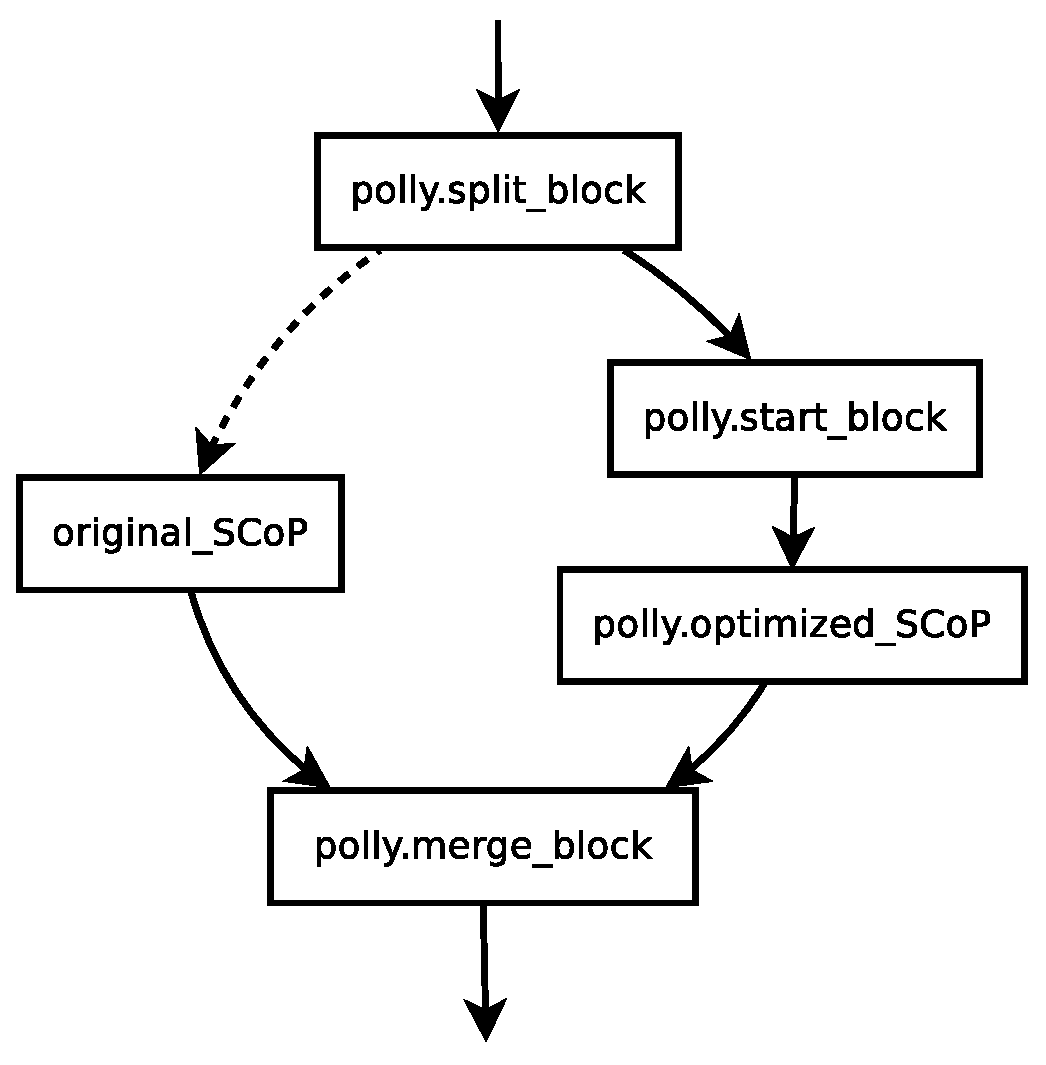
\includegraphics[width=0.9\textwidth]{Figures/PollySCoPCFG.eps}
    \label{fig:PollySCoPCFG}
    \end{minipage}
  }
  \subfloat[CFG after optimization with SPolly]{
    \begin{minipage}[c][1\width]{0.5\textwidth}
    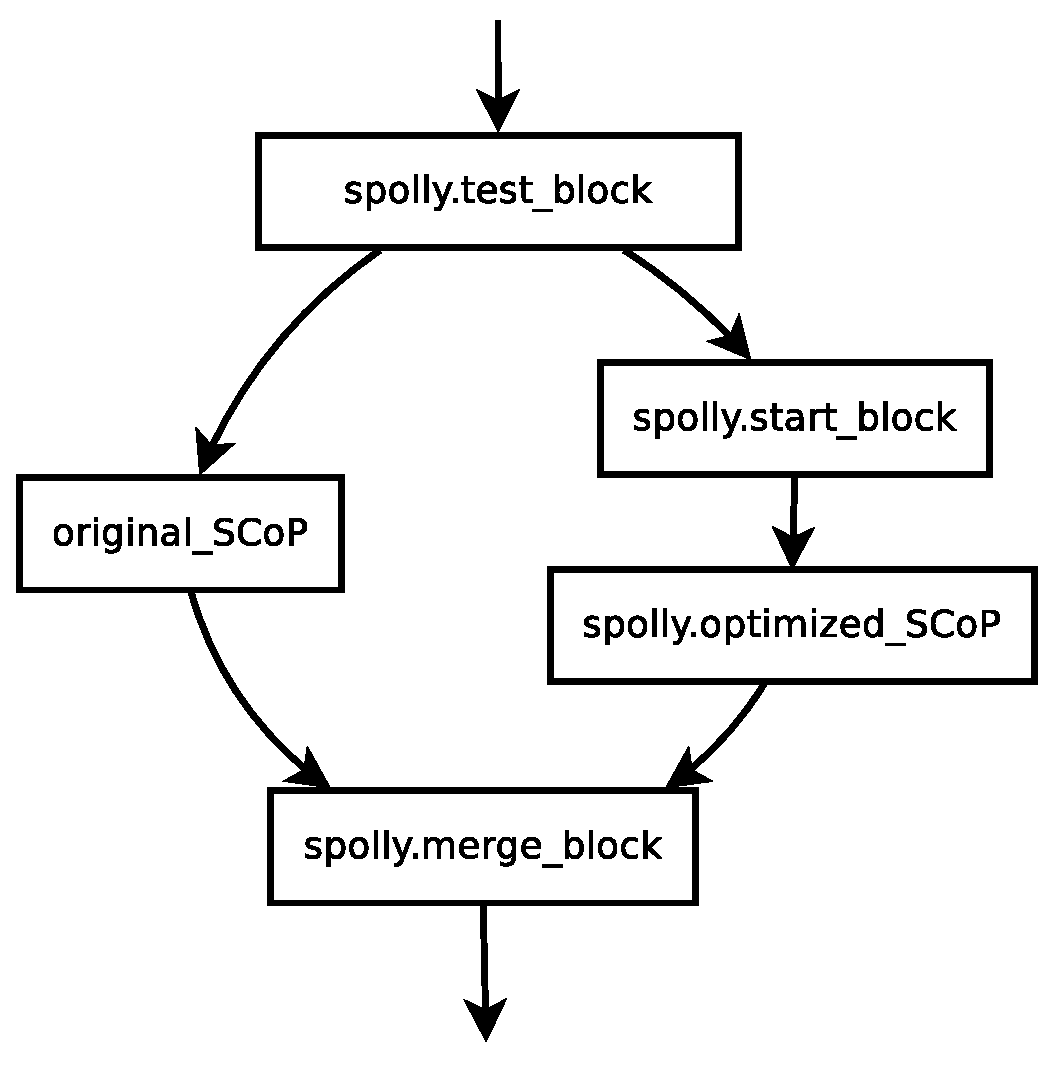
\includegraphics[width=0.9\textwidth]{Figures/SPollySCoPCFG.eps}
    \label{fig:SPollySCoPCFG}
    \end{minipage}
  }
  \caption{CFG produced by Polly and SPolly, respectively}
  \label{fig:SCoPCFG}  
\end{figure}





\subsection{Alias Tests}
Testing for aliasing pointers in general would not be feasible so another way 
was chosen. Only sSCoP invariant pointers are tested once before the sSCoP is
entered. If the test succeeds, thus no aliases are found, the optimized version
is executed. At compile time the accesses for each base pointer are collected and
marked either as possible minimal, possible maximal or not interesting access. At 
runtime all possible minimal and maximal accesses are respectively compared until,
in the end, the minimal and the maximal access for each base pointer is computed.
The alias test as such compares again the minimal access for a base pointer with the maximal 
accesses for each other base pointer and vice versa. After this comparison chain the 
result may indicate or rule out aliasing between them. As Polly introduces two 
versions of a SCoP by default, we may just replaces the constant guard in the
split block in order to choose the executed version based on the test result.
If all base pointers are invariant in the SCoP the test is complete,
thus aliasing can be ruled out for the sSCoP at runtime.
However, non invariant pointers are not tested at all, as it would 
imply to perform all computation and testing within the loop. 
Figure \ref{fig:AliastestConcept} illustrates the concept of the alias
tests while listing \ref{lst:AliastestAccessesSrc} and figure
\ref{fig:AliastestAccesses} provide an example loop nest and the corresponding 
minimal and maximal memory accesses. 
The alias test for this example would look like listing
\ref{lst:AliastestAccessesOut}.

\lstset{frame=none}
\begin{figure}[htbp]
  \centering
  \subfloat[Alias test from a birds eye view]{
  \begin{minipage}[c][4cm]{\textwidth}
    \includegraphics[width=0.9\textwidth]{Primitives/aliastest.eps}
  \end{minipage}
  \label{fig:AliastestConcept}  
  }

  \vspace*{5mm}
  \subfloat[Aliasing accesses]{
    \begin{minipage}[c][4cm]{0.5\textwidth}
    \lstinputlisting{Primitives/Code/aliastestbsp.c}
    \end{minipage}
    \label{lst:AliastestAccessesSrc}  
  }
  \subfloat[Statically derived min/maximal accesses]{
    \begin{minipage}[c][4cm]{0.4\textwidth}
    \vspace*{-2mm}
    \centering
    \begin{tabular}{ c c c c }
      Acc & bp & ma & Ma \\
      \hline
      I1 & C & 0 & N$ * $N$ - 1$ \\ 
      I2 & C & 0 & N$ * $N$ - 1$\\ 
      I3 & A & 0 & N$ * $N$ - 1$\\ 
      I4 & B & 0 & N$ * $N$ - 1$\\ 
    \end{tabular}
    \end{minipage}
    \label{fig:AliastestAccesses}  
  }
  
  \subfloat[Introduced compare chain]{
      \lstinputlisting{Primitives/Code/aliastestout.c}
    \label{lst:AliastestAccessesOut}  
  }
  \caption{Alias tests concept and example}
  \label{fig:Aliastest}  
\end{figure}
\resetlst





\subsection{Invariant Tests}
Apart from alias tests, SPolly may introduce invariants tests if there are
possibly invariant variables and a function call within a sSCoP. The key idea
is to monitor possible changes in such variables during the execution of the 
profiling version. As the results may introduce new dependencies 
between loop iterations, the sSCoP could be discarded. If it does not, the sSCoP
may be optimized, depending on its new region score. Even this is a 
disqualification test in the first place, the information gathered about the 
variables could be used to create specialized sSCoP versions too.
Listing \ref{lst:InvariantTestSRC} gives an example of an sSCoP 
for which invariant tests can be introduced and \ref{lst:InvariantTestOut} shows
the modified source. 

\lstset{frame=none}
\begin{figure}[htbp]
  \centering
  \subfloat[Loop nest with possible invariant variables]{
    \begin{minipage}[c][0.55\width]{0.45\textwidth}
    \lstinputlisting{Primitives/Code/InvariantTestSRC.c}
    \label{lst:InvariantTestSRC}
    \end{minipage}
  }
  \hspace*{5mm}
  \subfloat[Loop nest with invariant tests]{
    \begin{minipage}[c][0.55\width]{0.45\textwidth}
    \lstinputlisting{Primitives/Code/InvariantTest.c}
    \label{lst:InvariantTestOut}
    \end{minipage}
  }
  \caption{Invariant test introduced by SPolly}
  \label{lst:InvariantTest}  
\end{figure}
\resetlst






%\section{Irreversible Function Calls}
%Parallelizing loops containing function calls is a challenge on its own. 
%The called functions may have not computable side effects or they might just 
%print something on your screen. In both cases the ordering is important and 
%parallel execution becomes unlikely especially if these calls are placed on all
%execution paths. On the contrary there are loops which will execute such
%calls only rarely e.g., as part of error handling. SPolly locates all calls and
%allows loops which execute them only under certain conditions.
%[TODO gefaellt mir nich]






\section{Non Computable Dependencies}
\label{NonComputableDependencies}
Ruling out may aliases due to checks as described earlier is not feasible in every
situation. Assuming the example in listing \ref{lst:NonComputableDependenciesSrc}
we may check if \texttt{A} and \texttt{B} alias in front of the loop nest, but
every array \texttt{A[i]} and \texttt{B[i]} may alias also. Introducing tests 
within the loop nest is possible, but it would reduce the possible parallelism
to outermost loop not containing the aliases. As in the presented example type
based alias analysis could lift the computation of \texttt{A[i]} and \texttt{B[i]} 
to the outer loop, the innermost one would become a valid SCoP after checks are
introduced. At the moment SPolly is not capable of detection and deciding if 
such an approach could be profitable, but instead SPolly tries to optimize and 
speculate on the whole loop nest. As described earlier SPolly will overestimate
the data dependencies in order to apply sound transformations before it will 
speculatively execute the splitted loop nest in parrallel. This example is well
suited to illustrade why even an STM based approach cannot detect all conflicts
when no commit order is available. Assuming we would 
translate the loop to the pseudo parallelized version in listing 
\ref{lst:NonComputableDependenciesBad} with the corresponding ParCFG as illustrated 
by figure \ref{fig:NonComputableDependenciesParCFG}. An input such as the one 
in figure \ref{fig:NonComputableDependenciesSituation} seems very unlikely but 
nevertheless it could produce wrong results without causing an syncronizing 
conflict. This will happen everytime the second transaction is commited and 
therefor written first. This will cause the first one to recompute its results, 
because they worked on the same memory locations, namely the array \texttt{A[0] = A[1]}.
During this recomputation a wrong value for \texttt{A[0][j]} will be used without
beeing reported as a conflict on the syncronization. 

\lstset{frame=none}
\begin{figure}[htbp]
  \centering
  \subfloat[Loop nest with non computable dependencies]{
    \begin{minipage}[c][45mm]{0.45\textwidth}
    \lstinputlisting{Primitives/Code/NonComputableDependencies.c}
    \end{minipage}
    \label{lst:NonComputableDependenciesSrc}  
  }
  \subfloat[Possible input situation for listing \ref{lst:NonComputableDependenciesSrc}]{
    \begin{minipage}[c][45mm]{0.5\textwidth}
    \hfill\hfill
    \includegraphics[width=0.8\textwidth]{NonComputableDependenciesSituation.eps}
    \hfill\hfill
  \end{minipage}
  \label{fig:NonComputableDependenciesSituation}  
  }
  
  \subfloat[Loop nest \ref{lst:NonComputableDependenciesSrc} pseudo parallelized]{
    \begin{minipage}[c][80mm]{0.45\textwidth}
    \lstinputlisting{Primitives/Code/NonComputableDependenciesBad.c}
    \end{minipage}
    \label{lst:NonComputableDependenciesBad}  
  }
  \subfloat[ParCFG for listing \ref{lst:NonComputableDependenciesBad}]{
    \begin{minipage}[c][80mm]{0.5\textwidth}
    \hfill\hfill
    \includegraphics[width=0.8\textwidth]{NonComputableDependenciesParCFG.eps}
    \hfill\hfill
  \end{minipage}
  \label{fig:NonComputableDependenciesParCFG}  
  }

  \label{fig:NonComputableDependencies} 
  \caption{Example for non computable dependencies and a violating input}
\end{figure}
\resetlst





\subsection{Overestimating Dependencies}
\label{OverestimatingDependencies}
To handle loop nests with unknown dependencies, a conservative approach which 
pretends dependencies between all possibly aliasing instructions is already 
implemented.
The strategy is quite similar to the one Polly uses for non 
affine memory accesses as both overestimate the access until it is sound to 
proceed. This technique is quite restrictive but even though it may allow
loop invariant code motion or even vectorization. 

Considering listing \ref{lst:NonComputableDependenciesSrc} again this method 
will hoist the conditional out of the loop and at the same time reveal that
the innermost one has no loop carried dependencies. 





\section{What Is Missing}

%\section{}




